\newpage
\section{Třídy}

O logickou část Workflow Builderu se starají třídy Graph reprezentující graf, SubGraph reprezentující podgraf, Module reprezentující modul, Connection reprezentující spojení a Port reprezentující parametr modulu. Na diagramu \figurename \ref{logClass} je znázorněný vztah po vytvoření podgrafů (souvislých komponent) v grafu. Existuje vždy právě jedna instance třídy \textbf{Graph}. Tato instance může obsahovat libovolné množství instancí třídy \textbf{SubGraph}. Každá tato instance obsahuje minimálně jednu instanci třídy \textbf{Module}, dále může obsahovat instance třídy \textbf{Connection}. \textbf{Module} může obsahovat instance tříd \textbf{Port}, \textbf{Connection} a právě jednu instanci třídy \textbf{SubGraph}. Spojení v sobě drží informaci o počátečním a koncovém parametru a modulu.

\begin{figure}[h]
	\begin{center}takto
		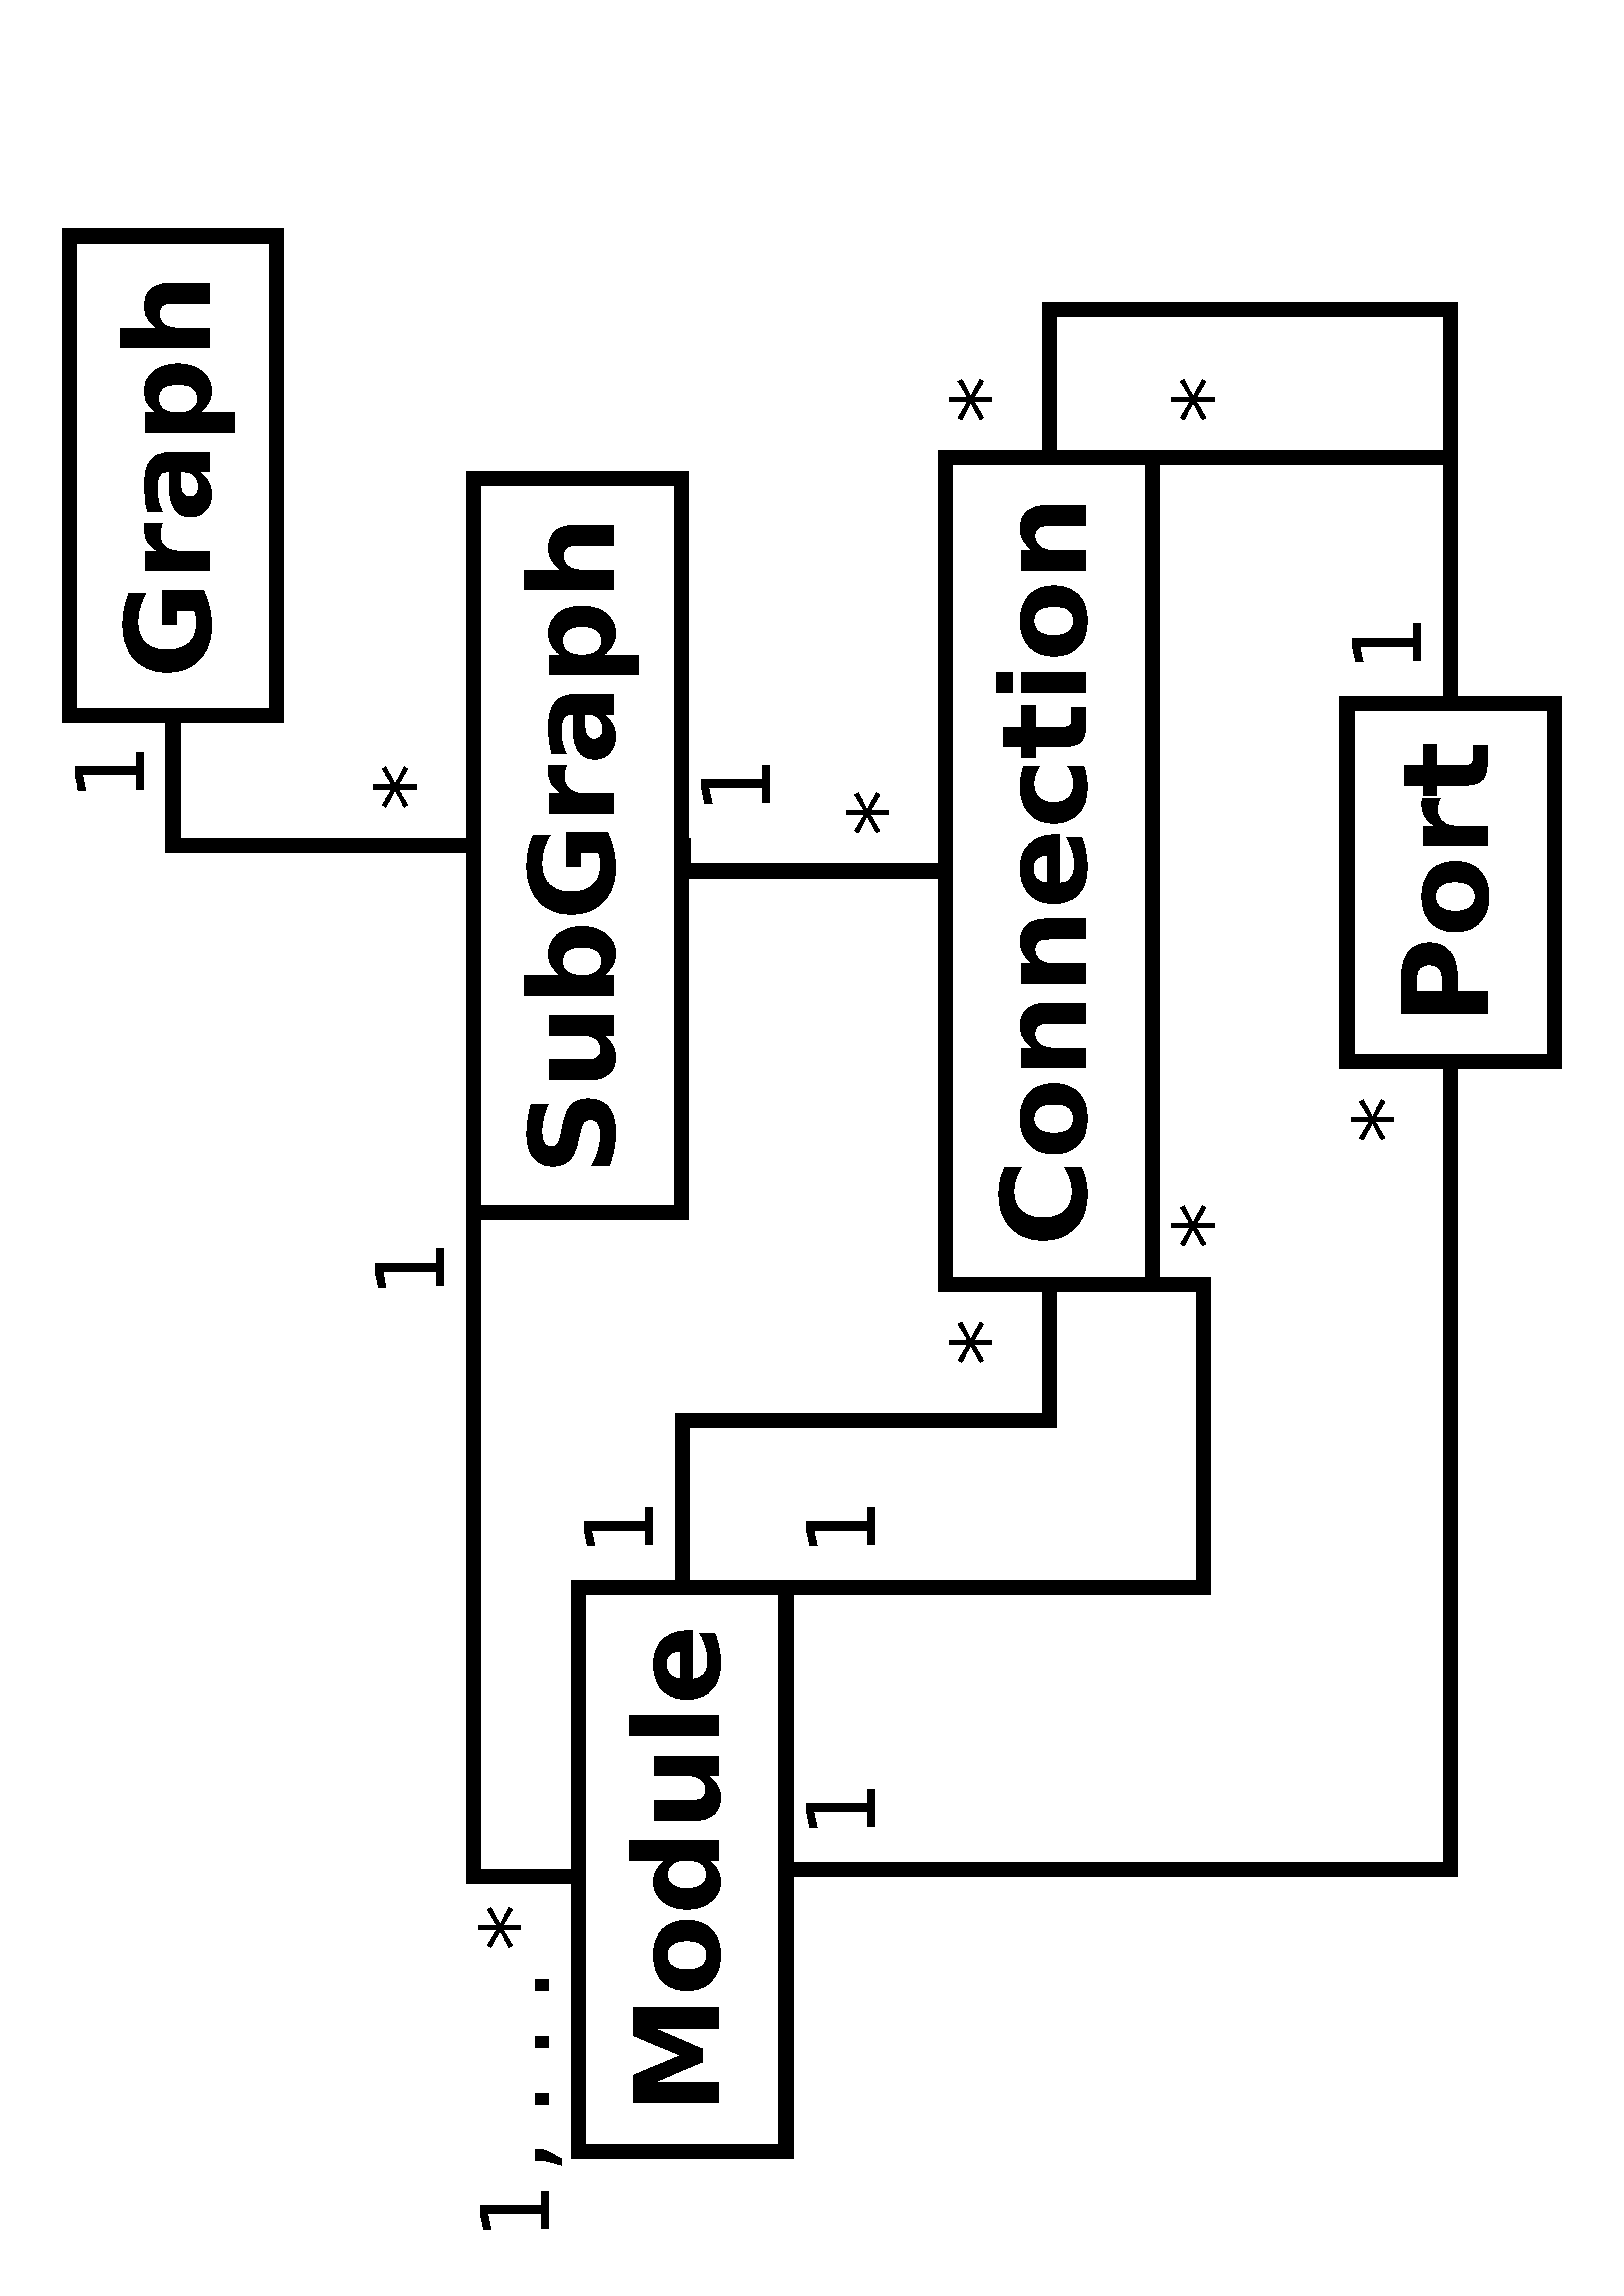
\includegraphics[scale=0.05,angle=-90]{pictures/wf/logClass.pdf}
		\caption{Diagram znázorňující vztahy mezi třídami Graph, SubGraph, Connection, Module a Port}
	  	\label{logClass}
	\end{center}
\end{figure}

Dialogové okno je instance třídy \textbf{WorkflowBuilder}, která je potomkem třídy \textbf{QDialog} z knihovny Qt. WorkflowBuilder se skládá z \textbf{GraphicsView} (reimplementace třídy QGraphicsView z Qt). GraphicsView zobrazuje prvky skrze scénu (\textbf{DiagramScene} - potomek QGraphicsScene z Qt). Třídu Module reprezentuje ve scéně třída \textbf{QGraphicsModuleItem}, třídu Connection třída \textbf{QGrahicsConnectionItem} a parametry jsou reprezentovány \textbf{QGraphcisPort}.

\begin{figure}[h]
	\begin{center}
		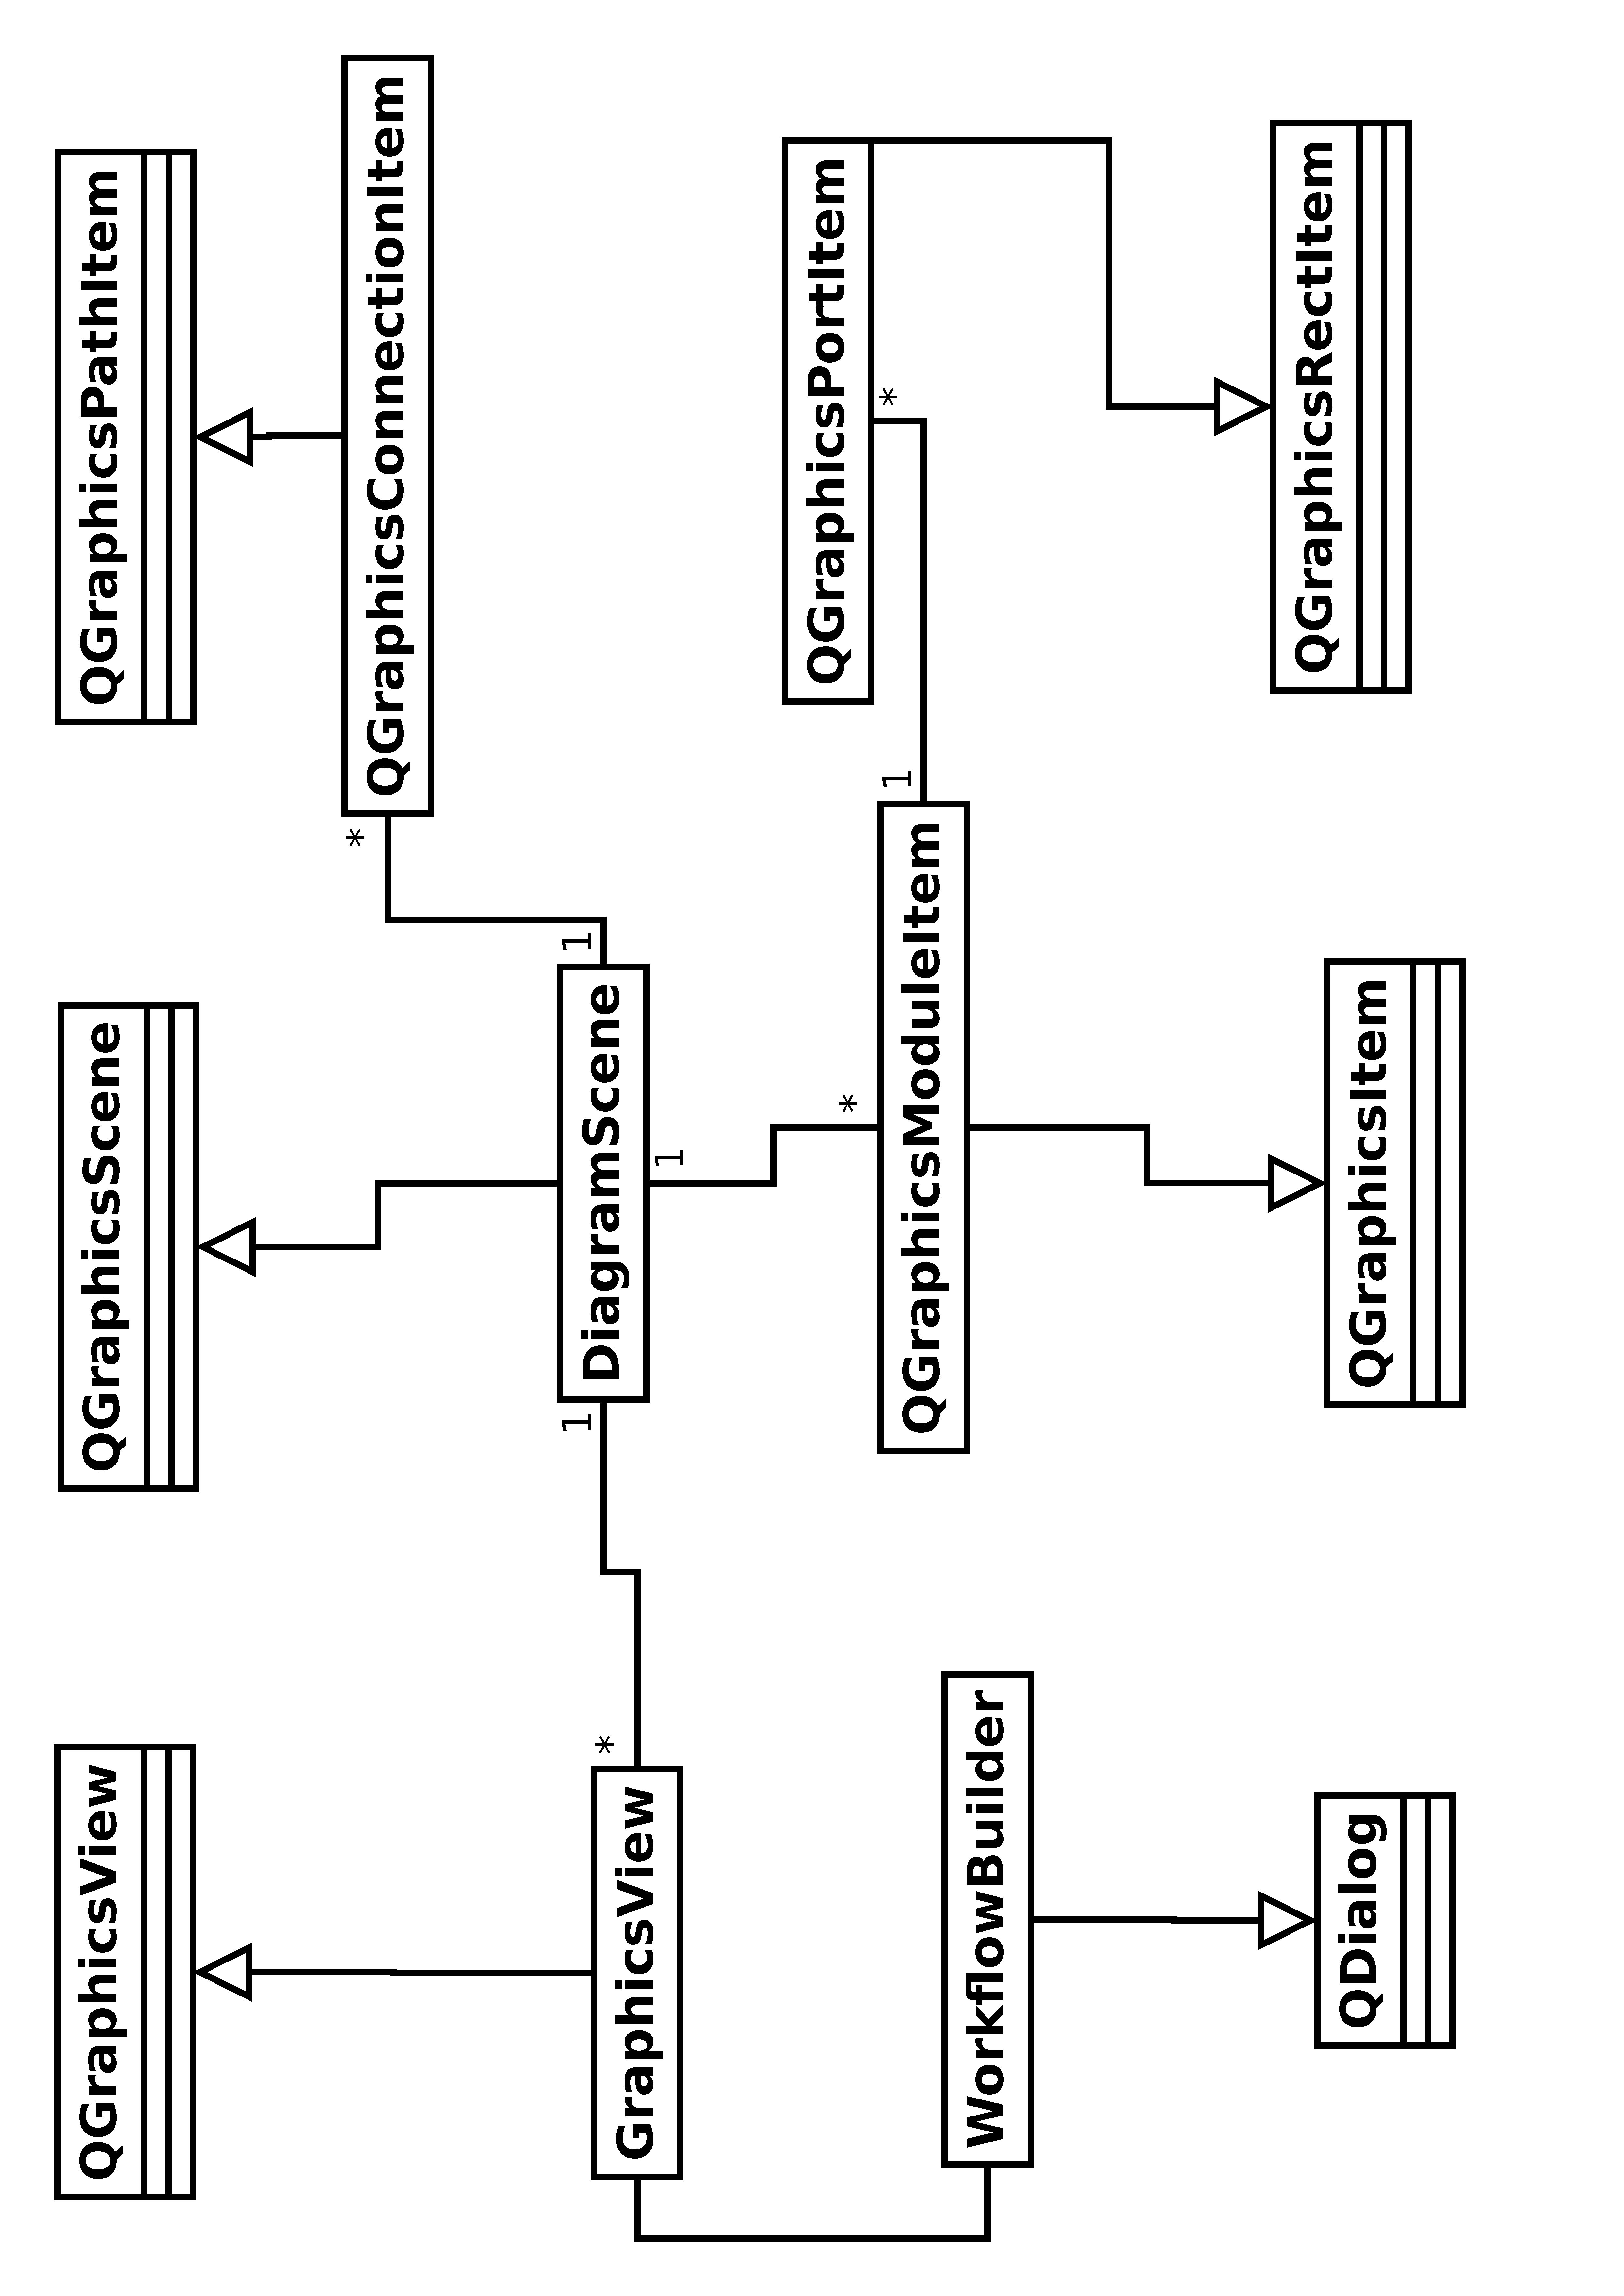
\includegraphics[scale=0.1,angle=-90]{pictures/wf/graphClass.pdf}
		\caption{Diagram znázorňující vztahy mezi třídami GraphcisView, GraphicsScene, QGraphicsModuleItem, QGraphicsConncetionItem a QGraphicsPortItem v třídě WorkflowBuilder}
	  	\label{graphClass}
	\end{center}
\end{figure}


\subsection*{Třída Graph}
Třída Graph je v podstatě samotné workflow. Obsahuje všechny moduly a spojení, které se ve workflow vyskytují. Hlavní metody jsou $executeGraph$() a $save$(). Metoda $executeGraph$() postupně prochází všechny podgrafy a jsou-li validní a neobsahují cyklus, spouští jejich moduly. Validní podgraf je ten, u jehož každého modulu jsou všechny vstupní parametry buď nastaveny nebo spojeny s jiným. Metoda $save$() vytvoří xml soubor reprezentující nový modul a obsahující všechny podgrafy, moduly a spojení. Metoda $addConnection$() přidá do grafu spojení, $addModule$() přidá do grafu modul, $addSubGraph$() přidá do grafu podgraf, $findLoop$() prochází graf a vrací True, najde-li v grafu cyklus, $xml$() vytvoří DOM reprezentaci grafu.

\subsection*{Třída SubGraph}
V řeči teorie grafů instance třídy \textbf{SubGraph} reprezentují souvislé komponenty grafu. V našem případě se jedná o instanci třídy \textbf{Graph}, která reprezentuje workflow.

Hlavní metody jsou $executeSGraph$() a $xml$(). Metoda $executeSGraph$() spouští všechny moduly v podgrafu. Metoda $xml$() je důležitá při ukládání nového modulu do souboru, vytvoří DOM reprezentaci podgrafu. Metody $prepareToExecute$() a $findLoop$() se spouští před samotným spuštěním podgrafu. $prepareToExecute$() prochází všechny moduly a zjišťuje, zdali jsou u každého modulu nastaveny vstupní parametry či jsou spojeny s jiným parametrem. Pakliže jsou, označí podgraf jako validní pomocí metody $setValid$(). Metoda $findLoop$() slouží k nalezení cyklu v daném podgrafu. 
%processing.framework[self.label].instance()
Pomocí metod $addModule$() a $setConnections$() přidáme do podgrafu modul, resp. nastavíme spojení.

\subsection*{Třída Module}
Třída Module reprezentuje PF Module v prostředí Workflow Builderu. Instance třídy v sobě uchovávají jméno, popis, tagy a parametry PF Modulu. Parametry se uchovávají v podobě instance třídy Port. 

Důležité jsou metody $getInstancePF$(), $execute$() a $xml$(). Metoda $getInstancePF$() vrací již nastavenou instanci třídy PF Module, která koresponduje s modulem z Workflow Builderu. Pakliže u modulu ještě nebyla vytvořena instance PF Modulu, vytvoří ji pomocí $processing.framework[nazev\_modulu].instance()$. \textbf{Port}ům modulu nastaví odkazy na parametry právě vytvořené instance třídy PF Module. 

Metoda $execute$() nastaví instanci PF Modulu parametru podle aktuálních hodnot \textbf{Port}ů modulu a spustí instanci PF Modulu. Potom nastaví hodnoty výstupů z PF Modulu do \textbf{Port}ů modulu a dále nastaví hodnoty i u \textbf{Port}ů, které jsou s daným výstupem (Portem, parametrem) spojené. 

Metoda $xml$() vytvoří DOM reprezentaci Modulu, která slouží pro uložení celého workflow do souboru formátu xml.

Instance třídy Module je jednoznačně identifikovatelná pomocí jejího identifikačního čísla, které je v rámci grafu (Graph) jedinečné.

Instance třídy \textbf{Module} jsou ve scéně reprezentována instancemi třídy \textbf{QGraphicsModelItem}.

\subsection*{Třída Port}  
Instance třídy \textbf{Port} reprezentují parametry PF Modulu. Jsou jednoznačně identifikovatelné pomocí identifikačního čísla, které je v rámci modulu jedinečné a pomocí identifikačního čísla modelu.

Uchovává v sobě informace jako název parametru, typ, zdali je parametr volitelný či povinný, zdali je parametr výstupní či vstupní, popis nebo výchozí hodnotu. Po úspěšném spuštění modulu a v případě, že je \textbf{Port} výstup, uloží se také nová hodnota.

Pomocí metody $getValue$() získáme aktuální hodnotu, metoda $outputData$() vrací výstupní data, $destinationPorts$() vrací porty, které jsou s daným portem spojené a ve spojení jsou vedeny jako cílové, $getToolTip$() vrací textový řetězec sloužící jako nápověda pro daný port, $isConnected$() vrací zdali je daný port spojen s jiným a $xml$() vrací DOM reprezentaci portu. Je-li \textbf{Port}, výstupní pomocí metody $addItToCanvas$() zjistíme, zdali si uživatel přál načíst vrstvu po spuštění modulu do QGIS, a metoda $outputName$() nám vrátí jméno, pod kterým se má vrstva načíst.

Instance třídy \textbf{Port} jsou ve scéně reprezentovány instancemi třídy \textbf{QGraphicsPortItem}.

\subsection*{Třída Connection}
Třída \textbf{Connection} v terminologii teorie grafů reprezentuje hrany. Uchovává v sobě informaci o počátečním a koncovém modulu (Module), resp. parametru (Port). A obsahuje jedinou metodu xml(), která vrací DOM reprezentaci spojení.

Instance třídy \textbf{Connection} jsou ve scéně reprezentovány instancemi třídy \textbf{QGraphicsConnectionItem}.

\subsection*{Třída GraphicsView}
Třída \textbf{GraphicsView} je reimplementací třídy \textbf{QGraphicsView} z knihovny Qt. Byla reimplementována metoda $wheelEvent$(), která umožňuje funkci zoom, a  metody $dragEnterEvent$(), $dragMoveEvent$() a $dropEvent$() pro spravování událostí týkajících se prostředí Drag and Drop. \textbf{GraphicsView} přijímá pouze objekty z Processing Manageru. Metoda $keyPressEvent$() je reimplementována tak, aby se po stisknutí klávesy $Delete$ smazaly všechny vybrané prvky. 


\subsection*{Třída DiagramScene}
Třída \textbf{DiagramScene} je reimplementací třídy \textbf{QGraphicsScene} z knihovny Qt. Byly reimplementovány metody mousePressEvent(), mouseMoveEvent() a mouseReleaseEvent(). Tyto metody řeší, zdali uživatel pouze kliknul na modul a chce, aby se mu zobrazili informace o parametrech, či kliknul na parametr a chce jej spojit s jiným. Také se zde řeší, zdali mohou být parametry spojeny. Pakliže ano, vytvoří se spojení (instance třídy Connection) a na jeho základě také instance třídy QGraphicsConnection.

dopsat
addModule
addConnection
delModule
delConnection
clearDockPanel
